%Profiler document
\documentclass[11pt,]{article}

\usepackage[top=2.54cm, bottom=2.54cm,left=1.27cm,right=1.27cm]{geometry}
\usepackage{graphicx} 
\usepackage{cite}
\usepackage{setspace}
\usepackage{listings}
\begin{document}
\begin{singlespace}
\title{Profiler Report and Timing Report for Lab07}
\author{Naveen Sagar\\120050026 ,
 \texttt{120050026@cse.iitb.ac.in} \\
\and
Aditya Kumar Akash\\120050046 , \texttt{adityaakash@cse.iitb.ac.in} \\ 
\and
Prateek Chandan\\120050042 , \texttt{prateekchandan@cse.iitb.ac.in} \\
}
\date{\today}
\maketitle 
\section{Introduction}
This Report aims to describe the profiling and timing behaviour of running of the Code. It contains explanation of the plots generated in Lab5
 and the explanation of profiling done in present lab
\section{Analysis Report from Lab05}
This section contains the Reports , Obsevations and Inference from the timing diagram which are obtained from the data and the 
Plots generated in lab5.\\
No of Iteration for which the 	the iteration was run for 1 to 150 and 15 rerun for each iteration
\subsection{Observation from Plot1}
The following inference were drawn from the Plot1 diagram which was Plot of Average Step time  and Average loop time:
\begin{enumerate}
    \item The Average loop time is greater than the Average Step Time but is almost equal
    \item The average time for the decreases as the no of iteration increases
\end{enumerate}
\textbf{Explanation:}
Since for the first few iterations the world is being set and all the objects in a state of movement to get settled to there stable state
and also the no of of collisions taking place are too high, the time taken by the Loop in fisrt few Interation are High.
But as he loop progresses the animation gradually takes place without much calcualtion or updates and the updates are very few so the time for 
the further loops decreases. Due to this the average time for more iterations decreases as compared o lesser no of Iterations\\

Since the step time is the of all times taken by the loop while the loop time is the total time taken by the loop in addition to the Time 
taken by system processes so the loop time is slightly greater than the step time. And when the same was generated while the sytem was overloaded 
with programs, This gap was still greater.
\begin{figure}[!ht]
	\centering
	\caption{Plot1}
		\includegraphics[scale=0.5]{../plots/g17_plot01.png}
\end{figure}
\subsection{Observation from Plot2}
The following inference were drawn from the Plot2 diagram which was Plot of Step time , Collision time , Velocity update time , Position update time
and sum of last 3 averaged:
\begin{enumerate}
    \item The step time is greater than the sum of Collision time , velocity update time and position update time
    \item All of these times decreases as the no of iteration increases
\end{enumerate}
\textbf{Explanation:}
The step time is the time taken by the loop which is running the Animation. But the other three times are exactly what they are meant to be.
But since the step time is the time taken by all of the things within a loop , So there are other processes which will also be called within the for loop 
and they will take time increasing the step tme\\

The explnation for initial times to be greater as the explanation in of Plot1
\begin{figure}[!ht]
	\centering
	\caption{Plot2}
		\includegraphics[scale=0.5]{../plots/g17_plot02.png}
\end{figure}
\subsection{Observation from Plot3}
The plot3 was the plot of averaged step time along with error bars calculated with standard deviation\\

It is observed that the error bars for the average stem time for lower no of iterations was too high as compared to the error
 bar for higher no of iterations \\
 
This might be because of the reasons explained in Plot1. Since the setting of world can take place differently for only one iteration because of 
setting up of worlds and setting up of initial position of objects so the error bar is too high. But when the no of iteration is high, This total 
time sums up to almost be equal. So the standard deviation is low making the error bar to be small. 
\begin{figure}[!ht]
	\centering
	\caption{Plot3}
		\includegraphics[scale=0.5]{../plots/g17_plot03.png}
\end{figure}
\subsection{Observation from Plot4}
The following inference were drawn from the Plot4 diagram which was the frequency and cumulative frequency plot for the step Time
\begin{enumerate}
    \item The Frequency for the average step time is highest at 0.94ms
    \item The Frequency starts increasing from time 0.84 ms and increases till 0.97 ms 
    \item Apart from these times there is a high frequncy for the time of around 1.04 ms
\end{enumerate}
\textbf{Explanation:}
Due to the reasons explained above When the step time gets averaged up it keeps fluctuating around the the average value which comes out to be 
0.94 second and the rest of the times are around it.\\

But there is an Outlier time of 1.04ms which denotes the time at the start of the loop. Since  At the beggining the times are higher so they 
contribute for a frequency of a higher time
\begin{figure}[!ht]
	\centering
	\caption{Plot4}
		\includegraphics[scale=0.5]{../plots/g17_plot04.png}
\end{figure}
\subsection{Observation from Plot5}
Plot 5 was the plot for the best fit line for the step time averaged over all data and step time averaged over some random data
\begin{enumerate}
    \item The points for the averaged time of all data and random data are almost equal 
    \item The best fit line comes to be almost same for both of them
\end{enumerate}
\textbf{Explanation:}
	Since the time for a particular iteration is almost the same so it doesnt matter much if the points are averaged over all data or 
the  points are averaged over only few random data. Due to this the points comes to be nearly the same and also the best fit line is nearly 
the same
\begin{figure}[!ht]
	\centering
	\caption{Plot5}
		\includegraphics[scale=0.5]{../plots/g17_plot05.png}
\end{figure}
\subsection{Changes when the CPU was heavily loaded}
The same were generated with lots of application running simultaneously on the machine and the plots were generated. 
The following were the observations:
\begin{enumerate}
    \item Times for all the plots increased slightly upward but there was not much significant change. 
    \item The error bars in Plot3 were slightly increased
    \item The frquency plot was more distributed and shifted towards right
\end{enumerate}
These observations were near to what is expected.The time taken by other processes was distributing the time for the current program increasing
the time and uncertainity of the timing diagrams
\subsection{Difference between time and gettimeofday()}
After running a few instances of code with gettimeofday and time command we observer following output:
\begin{enumerate}
    \item With CPU less loaded\\
		Total loop time is 12633.376953 ms\\
		real	0m12.643s\\
		user	0m12.623s\\
		sys	0m0.000s
    \item The CPU with some load\\
		Total loop time is 12993.852051 ms\\
		real	0m13.005s\\
		user	0m12.975s\\
		sys	0m0.008s
\end{enumerate}
Obsevations were a) The time of both the gettimeof day and time changes with CPU load, and b) The time from time command is slightly more than
gettimeofday \\

So both of them measures the time difference between two points which also depends ont he system processes running. But The time commnad also measures 
the time required for the loading of the binary files required for running of the executable and the time required for cleaning them up which is 
not there in gettimeofday function. So the time measured by gettimeof day is slightly more.



\subsection{Conclusion}
The "Intersting Things" Which are found in explaining these concepts were \\
Most Importantly the setting up of world and initial setting up of objects takes a lot of time letting the increase in initial times.\\
The heavy loading of CPU leads to increase in loop time denoting that the other processes slows down running of the program\\
Also it was interesting to find the difference between the time command and gettimeofday function
	
\newpage
\section{Profiling report of the code in different mode}
\subsection{Release mode and Debug Mode}
Debug and Release are different configurations for building a project.
 As the name implies, we generally use the Debug mode for debugging our project,
  and the Release mode for the final build for end users.\\
 \emph{The Debug mode} does not optimize the binary it produces (as optimizations can greatly complicate debugging), 
 and generates additional data to aid debugging.\\
 \emph{The Release mode} enables optimizations and generates less (or no) extra debug data. Turning on the optimization flags makes the compiler 
 attempt to improve the performance and/or code size at the expence of compilation time and the ability to debug the program.\\
 
 \emph{We have used perf profiler to make the profile data.}\\
 \emph{No of iteration for data : 10000}

\subsection{Call Graphs}
A call graph is a directed graph that represents calling relationships between subroutines in a computer program.
Specifically, each node represents a procedure and each edge indicates that procedure f calls procedure g.\\

\textbf{Generation of call graph using perf and the gprof2dot.py} \\
\begin{lstlisting}
perf record -g -- ./mybins/cs296_17_exe
perf report > g17_release_prof.dat
perf script | python gprof2dot.py -f perf | dot -Tpng -o release.png
\end{lstlisting}

\begin{figure}[h!]
	\centering
	\caption{Debug Call Graphs}
		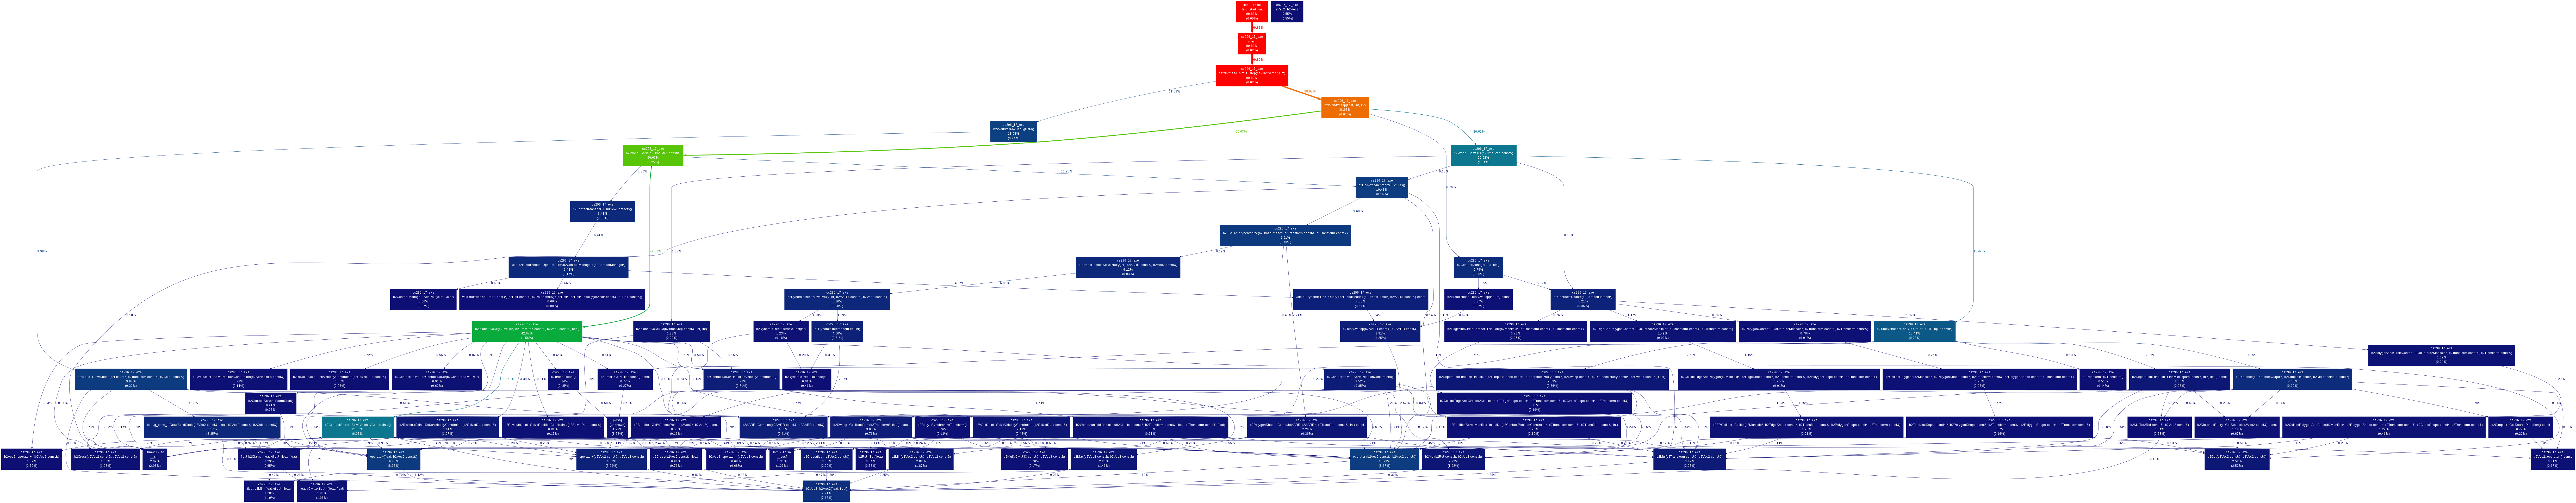
\includegraphics[width=1\textwidth]{debug.png}
\end{figure}

\subsection*{Observation from Debug Call Graph}
List of Functions which consume most time
\begin{enumerate}
    \item base\_sim\_t:step() 99.95 \%
    \item b2World::step() 88.85 \%
    \item b2World::solve() 58\%
    \item b2Island::solve() 38\%
    \item b2contactSolver::SolveVelocityConstraints() 19.22\%
    \item b2World::DrawShape() 10.35 \%
    \item b2World::DrawDebugData() 11.30 \%
    \item lib-2.17.so \_mcount 37.93 \%
    \item lib-2.17.so \_mcount\_internal 22.31 \%
\end{enumerate}

\begin{figure}[h!]
	\centering
	\caption{Release Call Graphs}
		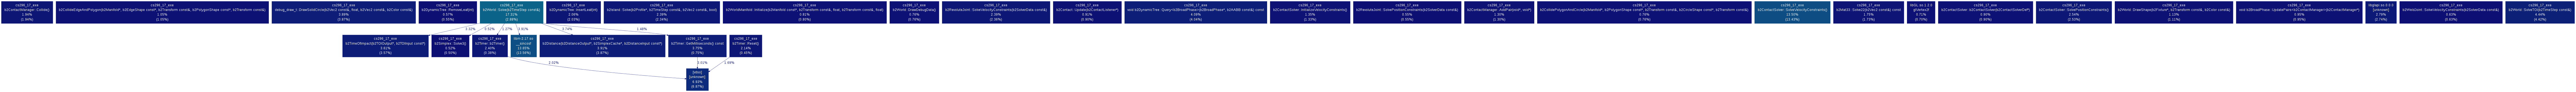
\includegraphics[width=1\textwidth]{release.png}
\end{figure}

\subsection*{Observation from Release Call Graph}
List of Functions which consume most time
\begin{enumerate}
    \item b2World::solve() 13.35\%
    \item b2contactSolver::SolveVelocityConstraints() 14.36\%
    \item b2World::DrawShape() 19.05 \%
    \item lib-2.17.so \_sincost 15.06 \%
    \item lib-2.17.so \_mcount 1.47 \%
    \item lib-2.17.so \_mcount\_internal 1.05 \%
\end{enumerate}

\subsection{Analysis of above Call Graphs}
\textbf{Debug Mode} :\\
As we can see from the callgraph and the most time consuming functions , debug mode calls much more functions as compared to the call graph of release mode.
Most of the time is consumed by the calculating functions which are solve , solveVelocityContraints etc and system library mcount (responsible for math calculations)
 consumes most of the time as compared to the Drawshape funstion and drawDebug function\\
\textbf{Release Mode} :\\
As opposed to the times in Debug mode , The Drawshape function take the most time in the running of the function while the solving function functions like
solveVelocityContraints and solve function took time much lesser than that in debug mode. also the system library used for calculation took very less
time 

\subsection{Inference from the above Analysis}
We can clearly see that the Debug mode is taking more time for all the functions in comparision to the release mode which does the optimization.\\
The function \emph{solveVelocityConstraint()} and \emph{solve()} takes more time in both the modes.
The step function is taking a lot of time in the debug mode as it is the function which is called again and again. \\
The \emph{DrawShape()} takes significant amount of time as this function is called each time the \emph{step()} function is called.
This function is responsible for updating the position of the various objects on the frame after the solving of all velocity and position 
constraint equation is solved. So it is natural for this function to take more time. \\
The library \_mcount takes more time in the debug mode but negligible amount in release mode and hence no need to optimize thus library.\\

\subsection{Optimizations Required}
We clearly see the effect of using the optimization in g++ compling option i.e the \textbf{use of -On option}. The inclusion of the option
provides various levels of optimizations such as the compiler tries to reduce code size and execution time, without performing any optimizations that take a great deal of compilation time. 
.GCC performs nearly all supported optimizations that do not involve a space-speed tradeoff. This increases both compilation time and the performance of the generated code.\\

But we also find that there are functions which still take major chunk of time in both modes. Thus these functions must be targeted to be \emph{optimized manually}.
From the analysis of the previous section we find that functions as - \textbf{\emph{solveVelocityConstraints(), solve() , DrawShape()}} are such functions 
which takes most times in both modes. Thus we have to find an efficient method to perform the operations performed by these functions such as 
solving the equations of position and velocity constraints.

\section{Conclusion}
The assignment helped to learn a great deal about use of profilers. The profilers help to generate the call graphs and thus visually identify the
part of code that consume more amount of time. As a result we get the capability of locate the part that if optimized would lead to better 
performance of code. So we can think of it as a great tool useful in situations where a huge code is to be optimized. \\

We also learnt the difference between comiple in release and debug mode and pros and cons of both.


\end{singlespace}
\end{document}
